\section{Usage}

\begin{frame}{Outline}
    \tableofcontents [current]
\end{frame}

\begin{frame}[containsverbatim] {Code sample}
\begin{Verbatim}[fontsize=\small]
#define LED_PIN 13

void setup () {
  // enable pin 13 for digital output
  pinMode (LED_PIN, OUTPUT);
}

void loop () {
  digitalWrite (LED_PIN, HIGH); // turn on the LED
  delay (1000); // wait one second (1000 milliseconds)
  digitalWrite (LED_PIN, LOW); // turn off the LED
  delay (1000); // wait one second
}
\end{Verbatim}
\end {frame}

\begin{frame}{The IDE}
	\begin{center}
		\includegraphics<1> [width=1\textwidth,keepaspectratio] {img/ide_examples.png}
		\includegraphics<2> [width=1\textwidth,keepaspectratio] {img/ide_webserver.png}
		\includegraphics<3> [width=1\textwidth,keepaspectratio] {img/ide_webserver_buttons.png}
		\includegraphics<4> [width=1\textwidth,keepaspectratio] {img/ide_serial.png}
	\end{center}
\end{frame}

\begin{frame}{Stats}
	\begin{center}
		\includegraphics<1> [width=1\textwidth,keepaspectratio] {pdf/memory0.pdf}
		\includegraphics<2> [width=1\textwidth,keepaspectratio] {pdf/memory1.pdf}
	\end{center}
\end{frame}

\begin{frame} {Documentation}
	On the arduino.cc website
	\begin{itemize}
		\item Simple, Readable, Relevant 
		\item open access (and edit) wiki, 
		\item regular updates
	\end{itemize}
\end{frame}

\begin {frame} {Documentation}
	For all pages about a subject, there are
	\begin{itemize}
		\item hardware scheme
		\item code samples, with relevant comments, Creative Common license
	\end{itemize}
\end {frame}

\begin {frame} {Examples}
	\begin {center}
		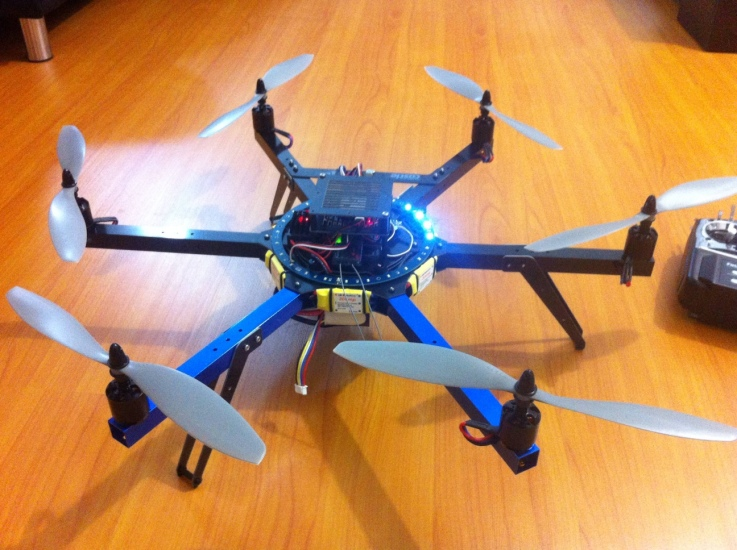
\includegraphics [width=.7\textwidth,keepaspectratio] {img/drone}
	\end {center}
\end {frame}

\begin {frame} {Examples}
	\begin {center}
		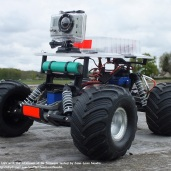
\includegraphics [width=.5\textwidth,keepaspectratio] {img/rover}
	\end {center}
\end {frame}
